\section{Optimal Block Size} \label{sec:res-blocksize}

One of the main determining factors for performance of a kernel is its launch configuration, which includes its grid size (number of blocks) and block size (number of threads, see section \ref{sec:hardware}). Cuda provides the option to specify block sizes in three dimensions, providing each thread with a X-, Y- and Z-index. In our benchmarks, we have tested all possible combinations of block sizes in steps of powers of two from 32 up to 512.

In order to cover the entire problem domain (which remains constant in size), a decrease in number of threads is always accompanied by an increase in the number of blocks (grid size), and vice versa. Owing to the way we map thread indices onto memory indices (X thread index maps onto memory index directly), thread sizes in the X-dimension of less than $32$ are highly inefficient. They lead to non-coalescing memory accesses. The X-dimension of the benchmarked block sizes is therefore always at least $32$.

\subsection{Overview}

The optimal \emph{total number} of threads depends mostly on the grid access implementation employed. In general, the same patterns can be observed for all three tested stencils and for all tested grid memory storage implementations: When using the \emph{naive}, \emph{idxvar} or \emph{shared} grid access strategies, it is best to have a high number of threads in total (256-512). The \emph{kloop} and \emph{kloop-sliced} thrive on a lower number of threads due to occupancy concerns. An exemplary overview of the runtimes as a function of total block size is given in figure \ref{fig:blocksizes-overview}.

\begin{figure}
	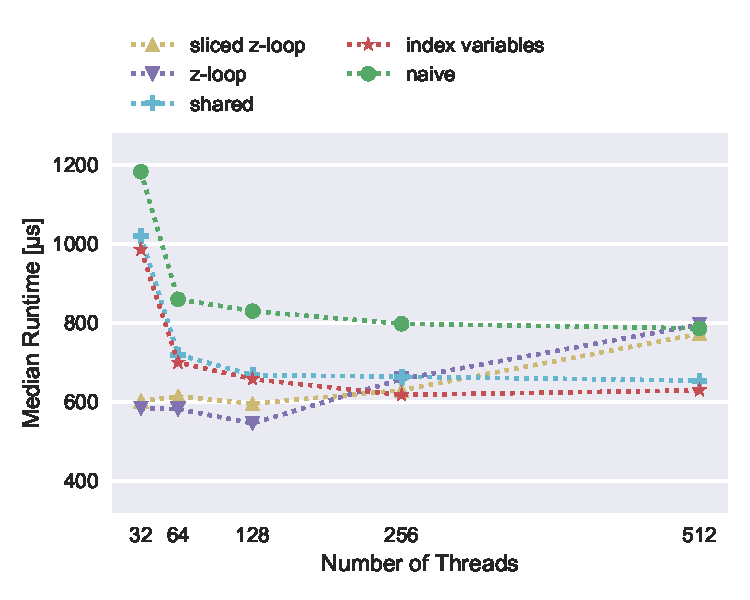
\includegraphics[scale=0.75]{laplap-z-curves-no-comp-chase-threads-prod.pdf}
	\caption{\label{fig:blocksizes-overview} Overview of the runtime for different implementations of the \emph{laplap} stencil on a $512\times 512\times 64$-sized domain (unstructured grid, pointer chasing, z-curves layout, uncompressed neighborship table) as a function on different total block sizes (product of X-, Y- and Z-blocksize). Results for other stencils and variants are of similar shape.}
	% ./plot.py -i results/ultimate.csv --size 16777216 -p line -x threads-prod --stencil laplap --z-curves z-curves --chase chase --comp no-comp  --marker variant --scale-min 400 --scale-max 1200 --plot-size 5 4
\end{figure}

The best \emph{shape} of the block size vector changes with the used grid storage strategy. Using \emph{uncompressed} neighborship tables, it is best for the \emph{naive}, \emph{idxvar} and \emph{shared} access strategies to have 32 or 64 threads in X-dimension and the rest in Z-dimension. Those implementations profit of more Z-threads because of the regularity of the grid in the Z-dimension. The \emph{non-chasing} variants profit even more of additional threads in the Z-dimension. This is due to the fact that in non-chasing variants, more neighborships are stored in the table; cache entries are thus evicted faster if many different X- and Y-coordinates are accessed. Switching to \emph{comepressed} neighborship tables, additional threads in the Z-dimension are of no use to any of the access strategies -- the reduced number of neighborship table entries after compression is accessed often enough to remain in cache independent of the Z-dimension of the block size. See figure \ref{fig:blocksizes-z} for a comparision of how changes in the Z-dimension of the blocksize vector translate to runtime changes. Whether the grid is stored as row-major or using z-order curves does not impact the required block sizes.

\begin{figure}
	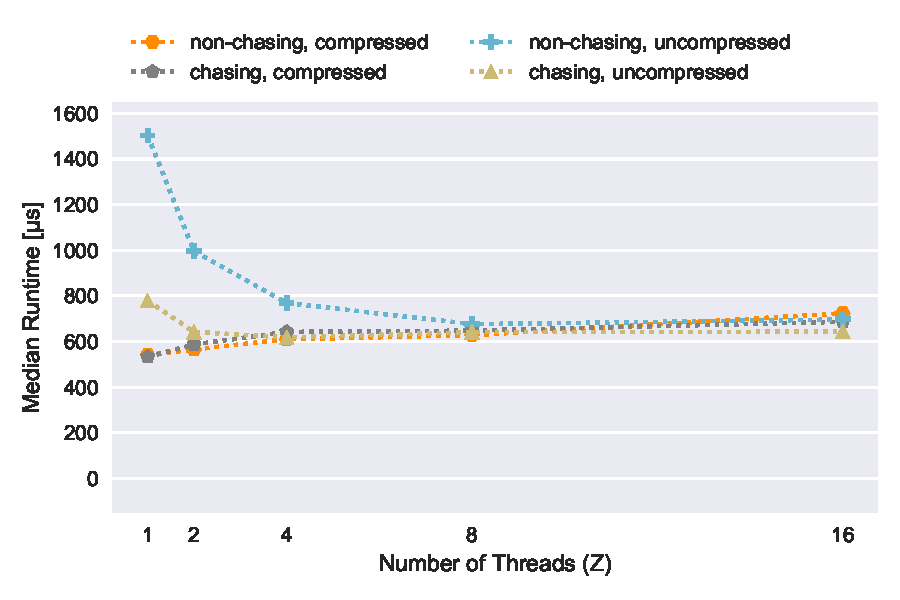
\includegraphics[scale=0.75]{laplap-zcurves-idxvar-threads-z.pdf} % ./plot.py -b unstr -i results/ultimate.csv --stencil laplap --variant idxvar --z-curves z-curves --size $((512*512*64)) --color storage --marker storage -p line -x threads-z -o results/blocksizes/laplap-zcurves-idxvar-threads-z.pdf --scale-max 1500
	\caption{\label{fig:blocksizes-z}Fastest runtimes for each fixed number of threads in the Z-dimension (other dimensions free) for the \emph{laplap} stencil on a $512\times 512\times 64$-sized domain (unstructured grid, row-major storage) for compressed and uncompressed variants, with and without pointer chasing.}
\end{figure}

\subsection{Optimal Block Sizes per Access Strategy}

\subsubsection{\emph{Naive}, \emph{Idxvar} and \emph{Shared} Grid Access Strategies}
In order to always cover the entire problem domain, the number of blocks $b$ in each dimension in the \emph{naive}, \emph{idxvar} and \emph{shared} grid access strategies is chosen as a function on the problem size $d$ and the chosen number of threads $t$ as follows:
$$b = \begin{pmatrix}\left\lceil\frac{d_x}{t_x}\right\rceil & \left\lceil\frac{d_y}{t_y}\right\rceil & \left\lceil\frac{d_z}{t_z}\right\rceil\end{pmatrix}^\top$$

For the \emph{naive}, \emph{idxvar} and \emph{shared} implementations, a high number of threads per block is beneficial to performance. For grids using an uncompressed neighborship table, increasing the number of threads in the Z-dimension especially improves performance.

For the \emph{naive} and \emph{idxvar} strategies, the advantage of multiple threads in Z (in grids using uncompressed neighborship tables) can be explained through the regularity of the unstructured grid in Z-direction: Cells with identical X and Y coordinates share the same entry in the neighborship table. By having multiple threads in a block operate on different Z-levels, caching of this neighborship table entry becomes very effective. Evidence for this presumed reason for the speedup is given by two facts: One, of all block size combinations tested, the ones with more threads in the Z-dimension perform best. Two, the Nvidia profiler reports higher cache hit rates if the number of threads in Z-dimension is increased. As an example of this for the \emph{idxvar} access strategy, see table \ref{tab:laplap-blocksize-metrics}.

These effects are strongest for grids that also store neighbors-of-neighbors in the neighborship table (no pointer chasing). As this leads to a larger number of entries in the neighborship table that are stored and accessed, entries may be evicted from the cache more quickly. More threads in the Z-dimension, which access the same neighborship table entries, prevent this.

At the opposite end of the spectrum lie the grids stored using compressed neighborship tables. These tables are much smaller, and the same few entries are accessed in almost all threads. Because of this, neighborship table entries remain in cache no matter the shape of the block size vector, and additional threads in the Z-dimension bring no benefit. Cache locality for the accessed values is more important here; depending on the used layout for the values (z-order-curves or row-major) this means adding additional threads in X (z-curves, spatial locality given), or X and Y (row-major, adding another thread in Y gives some spatial locality).

\begin{table}
%	\begin{tabular}{l l l l l}
%		Blocksize & \texttt{global\_hit\_rate} & \texttt{tex\_cache\_hit\_rate} & \texttt{l2\_tex\_read\_hit\_rate} & \texttt{l2\_tex\_hit\_rate} \\
%		\hline
%		$32\times 1\times 1$ & $45.42\%$ & $44.39\%$ & $73.86\%$ & $67.69\%$ \\
%		$32\times 1\times 2$ & $58.83\%$ & $57.96\%$ & $76.60\%$ & $68.12\%$ \\
%		$64\times 1\times 2$ & $62.25\%$ & $66.21\%$ & $69.99\%$ & $60.36\%$ \\
%		$64\times 1\times 4$ & $72.33\%$ & $71.72\%$ & $72.77\%$ & $60.81\%$
%	\end{tabular}
	\begin{tabular}{l l l l l}
		Blocksize & \texttt{tex\_cache\_hit\_rate} & \texttt{l2\_tex\_hit\_rate} \\
		\hline
		$32\times 1\times 1$ & $44.39\%$ & $67.69\%$ \\
		$32\times 1\times 2$ & $57.96\%$ & $68.12\%$ \\
		$64\times 1\times 2$ & $66.21\%$ & $60.36\%$ \\
		$64\times 1\times 4$ & $71.72\%$ & $60.81\%$
	\end{tabular}
	\caption{\label{tab:laplap-blocksize-metrics} Cache hit rates for different block sizes for the \emph{laplap} stencil using a \emph{idxvar} grid access strategy on a $512\times 512\times 64$-sized domain (unstructured grid, pointer chasing, stored in z-curves layout, uncompressed neighborship table)}
\end{table}

By the design of the \emph{shared} access strategy, a speedup is supposed to be attained with a larger number of Z-threads; if there are more threads in Z-dimension within a block, more sharing of neighborship relations through shared memory can take place. These implementations indeed profit from more threads through shared memory in much the same way as \emph{naive} and \emph{idxvar} variants profit from more threads through the cache in the uncompressed grids.

\subsubsection{\emph{Z-loop} and \emph{Z-loop-sliced} Grid Access Strategies}
Contrary to the other stencils, the \emph{z-loop} and \emph{z-loop-sliced} grid access strategies suffer from a high total thread count. As both of these strategies require one thread to perform calculations for multiple cells on different Z-levels, the total number of blocks and threads required to cover the entire grid is smaller. On the largest tested grid size ($512\times 512\times 64$), this leads to occupancy issues: As threads stall, there is not enough work can be scheduled to certain streaming multiprocessors to hide that latency. All threads inside a block are required to be executed on the same SM. Having more threads inside a block thus gives less blocks that can be scheduled onto stalled SMs. Smaller block sizes, on the other hand, give the scheduler a larger pool of blocks to choose from when trying to hide latency. Compare table \ref{tab:laplap-blocksize-occupancy} for an example of how a too large block size negatively impacts the \emph{kloop} implementation of the exemplary \emph{laplap} benchmark.

\begin{table}
	\begin{tabular}{l l l l l}
		Variant & Blocksize & Runtime & \texttt{achieved\_occupancy} & \texttt{issue\_slot\_utilization} \\
		\hline
		idxvar & $512$ & $783\mu s$ & $85\%$ & $19\%$ \\
		idxvar & $128$ & $844\mu s$ & $\mathbf{92\%}$ & $18\%$ \\
		idxvar & $32$  & $986\mu s$ & $48\%$ & $16\%$ \\
		z-loop & $512$ & $796\mu s$ & $25\%$ & $10\%$\\
		z-loop & $128$ & $\mathbf{546\mu s}$ & $42\%$ & $13\%$ \\ 
		z-loop & $32$  & $584\mu s$ & $41\%$ & $12\%$
	\end{tabular}
	\caption{\label{tab:laplap-blocksize-occupancy} Runtimes and occupancy metrics of \emph{idxvar} and \emph{z-loop} variant implementations of a \emph{laplap} stencil on an unstructured grid (size $512\times 512\times 64$, uncompressed neighborship table, z-curve memory layout, pointer chasing) for a selection of block sizes. The following block shapes were used: $512 = 256\times 2\times 1$, $128 = 64\times 2\times 1$ and $32 = 32\times 1 \times 1$. This highlights the occupancy issues the z-loop variant faces with too large block sizes. Note how the occupancy drops with increased number of threads for the z-loop variant, and how the runtime increases with it.}
\end{table}